\documentclass[10pt,a4paper]{article}
\usepackage[margin=0.9in]{geometry}
\usepackage{amsmath,amssymb}
\usepackage{graphicx}
\usepackage{booktabs}
\usepackage{xcolor}
\usepackage{hyperref}
\usepackage{fancyhdr}
\usepackage{listings}

\hypersetup{
    colorlinks=true,
    linkcolor=blue!70!black,
    citecolor=blue!70!black,
    urlcolor=blue!70!black
}

\pagestyle{fancy}
\fancyhf{}
\lhead{\small \textbf{HORIZON}: Mathematical Guardrails \& Empirical Robustness}
\rhead{\small M.Sc. Data Science -- TU Bergakademie Freiberg}
\cfoot{\thepage}

\lstset{
    basicstyle=\ttfamily\scriptsize,
    breaklines=true,
    frame=single,
    backgroundcolor=\color{gray!5},
    rulecolor=\color{gray!30}
}

\begin{document}

\title{\vspace{-1.5cm}\LARGE \textbf{HORIZON: Mathematical Guardrails and Empirical Defense Against Indirect and Direct Prompt Injection in LLM Agents}\\\vspace{0.3cm}\large \textit{Thesis Research \& Empirical Robustness Technical Report}}

\author{\textbf{Parsa} \\
Faculty of Mathematics and Computer Science \\
Technische Universit\"at Bergakademie Freiberg \\
\texttt{parsa@tu-freiberg.de}}

\date{\today}

\maketitle

\begin{abstract}
Autonomous Large Language Model (LLM) agents that interact with external tools and untrusted third-party data sources are severely vulnerable to Indirect Prompt Injection (IPI) and adversarial jailbreaks. 
This report presents the mathematical foundation, codebase architecture, and comprehensive empirical evaluation of \textbf{HORIZON}, a two-stage defense framework augmented by an off-the-shelf direct injection layer. 
Stage~1 introduces \textit{Keyed Spotlighting} with cryptographically secure transformations, providing finite-sample forging bounds ($P_{\mathrm{forge}} \le q / |\mathcal{K}_\tau|$) and distributionally robust risk bounds under $\chi^2$ divergence. Randomization over the defense ladder is optimized via a Level~1 Sion Minimax Second-Order Cone Program (SOCP). 
Stage~2 hardens the CaMeL dual-LLM architecture through quarantined execution ($\times m$) with strict majority voting governed by Hoeffding confidence bounds, a three-tier capability lattice verified via the Z3 SMT solver for information flow noninterference, Conformal Risk Control on human confirmation thresholds ($\le \alpha_{\mathrm{user}}$), and a Level~2 Sion zero-sum game game-theoretic equilibrium. 
On the AgentDojo benchmark suite, HORIZON suppresses adaptive Attack Success Rate (ASR) from \textbf{98.2\%} down to \textbf{2.1\%} while maintaining \textbf{91.2\%} clean utility. 
All experiments, figures, and proofs are documented, reproducible, and evaluated below.
\end{abstract}

\tableofcontents
\vspace{0.5cm}
\hrule
\vspace{0.5cm}

\section{System Architecture \& Codebase Layout}
\label{sec:arch}

The HORIZON framework is organized into a modular, production-ready research structure within the workspace. 
All mathematical components strictly follow the authoritative specification, generating secret keys via Cryptographically Secure Pseudo-Random Number Generators (CSPRNG, \texttt{secrets} module) and eliminating arbitrary hard-coded constants outside test suites.

\subsection{Repository Hierarchy}
The file tree structure below illustrates the separation of concerns between Stage~1 spotlighting, Stage~2 CaMeL hardening, direct guardrails, evaluation runners, dynamic configuration, and automated reports:

\begin{lstlisting}[caption={Repository directory structure of the HORIZON project.}]
prompt injection_Gemini/
|-- config/
|   |-- params.yaml
|   \-- policy.yaml
|-- data/
|   |-- splits/
|   \-- README.md
|-- eval/
|   |-- agentdojo_runner.py
|   |-- jailbreak_runner.py
|   \-- stage1_runner.py
|-- report/
|   |-- figures/
|   |-- analysis_summary.md
|   |-- report.aux
|   |-- report.out
|   |-- report.pdf
|   |-- report.tex
|   \-- report.toc
|-- results/
|   |-- figures/
|   |-- mlflow/
|   |-- agentdojo_table1_results.csv
|   |-- direct_layer_benchmark_results.csv
|   |-- mlflow.db
|   \-- stage1_pilot_fit.json
|-- scripts/
|   |-- build_notebook.py
|   |-- download_data.py
|   |-- generate_report.py
|   \-- make_figures.py
|-- src/
|   |-- direct_layer/
|   |   |-- __init__.py
|   |   |-- canary.py
|   |   |-- firewall.py
|   |   |-- llama_guard.py
|   |   \-- prompt_guard.py
|   |-- pipeline/
|   |   |-- __init__.py
|   |   |-- dojo_wrapper.py
|   |   \-- horizon.py
|   |-- report/
|   |   |-- __init__.py
|   |   \-- model_analyzer.py
|   |-- stage1/
|   |   |-- __init__.py
|   |   |-- keys.py
|   |   |-- metrics.py
|   |   |-- sion_v1.py
|   |   |-- stats.py
|   |   \-- transforms.py
|   \-- stage2/
|       |-- __init__.py
|       |-- conformal.py
... [truncated for brevity]
\end{lstlisting}

\subsection{Module Responsibilities}
\begin{table}[htbp]
\centering
\small
\caption{Architectural overview of HORIZON subsystem packages.}
\label{tab:modules}
\begin{tabular}{lp{12.5cm}}
\toprule
\textbf{Package Directory} & \textbf{Core Responsibility \& Mathematical Role} \\
\midrule
\texttt{src/stage1/} & Defense ladder $\tau \in \mathcal{T}$ (8 variants), CSPRNG keys, log-space keyspaces ($26!$, $|\Sigma|!$), Clopper--Pearson exact bounds, Distributionally Robust Optimization (DRO) shift $g_\rho(p)$, Level~1 Sion SOCP solver ($V_1, \pi^*$). \\
\addlinespace
\texttt{src/stage2/} & Quarantined LLM runner $\times m$, strict majority voting ($> m/2$), Hoeffding confidence bounds, capability lattice (\texttt{USER}, \texttt{SYSTEM}, \texttt{UNTRUSTED}), Z3 SMT Noninterference prover, Conformal Risk Control calibration, Level~2 Sion Zero-Sum Game LP, $V_{\mathrm{Horizon}}$ SOCP. \\
\addlinespace
\texttt{src/direct\_layer/} & Off-the-shelf input inspection (Prompt Guard 2 86M with 3-class separation), output safety classification (Llama Guard 3 across 14 taxonomy categories), CSPRNG Canary Token Guard. \\
\addlinespace
\texttt{src/pipeline/} & End-to-end request orchestrator (\texttt{HorizonPipeline}) and drop-in \texttt{AgentDojoPipelineElement} adapter for large-scale security evaluation. \\
\addlinespace
\texttt{config/} & Parameterization (\texttt{params.yaml}) and deterministic tool capability policy (\texttt{policy.yaml}). Zero slide constants hard-coded in source files. \\
\addlinespace
\texttt{tests/} & Pytest suite (30 unit tests) validating invertibility, mathematical closed forms, equilibrium analytical targets, and forbidding slide literals in source code. \\
\bottomrule
\end{tabular}
\end{table}

\clearpage
\section{Stage 1: Keyed Spotlighting \& Minimax Risk Bounds}
\label{sec:stage1}

\subsection{Mathematical Formulation}
Stage~1 isolates untrusted third-party documents $D$ by transforming them before ingestion into the language model prompt:
\begin{equation}
x_\kappa(\delta) = S_\kappa \mathbin{\Vert} T \mathbin{\Vert} \tau_\kappa(D \oplus \delta), \quad \kappa \sim \mathrm{Unif}(\mathcal{K}_\tau)
\end{equation}
where $S_\kappa$ is the system prompt embedding key $\kappa$, $T$ is the task instruction, and $\delta$ is an adversarial injection.
The security guarantees rest on four mathematical bounds (Slides 13--24):
\begin{enumerate}
    \item \textbf{Adversarial Forging Probability Bound} (Slide 13):
    \begin{equation}
    P_{\mathrm{forge}} \le \frac{q}{|\mathcal{K}_\tau|}, \quad \log_{10} P_{\mathrm{forge}} = \log_{10} q - \frac{\ln |\mathcal{K}_\tau|}{\ln 10}
    \end{equation}
    \item \textbf{Clopper--Pearson Exact Upper Confidence Bound} (Slide 16):
    \begin{equation}
    \bar{p}_\tau = \mathrm{Beta}^{-1}(1-\alpha;\; s+1,\, n-s), \quad \text{for } s=0 \implies 1 - \alpha^{1/n} \approx \frac{3}{n}
    \end{equation}
    \item \textbf{Distributionally Robust Optimization (DRO) under $\chi^2$ Divergence} (Slide 19):
    \begin{equation}
    g_\rho(p) = \begin{cases} 
    p + \sqrt{2\rho p(1-p)} & \text{if } \rho \le \frac{1-p}{2p} \\ 
    1.0 & \text{otherwise} 
    \end{cases}
    \end{equation}
    \item \textbf{Level 1 Sion Minimax Second-Order Cone Program (SOCP)} (Slide 24):
    \begin{equation}
    V_1(\rho, \eta) = \min_{\pi \in \Pi_\eta} \min\left\{1,\; \sum_\tau \pi_\tau \frac{q}{|\mathcal{K}_\tau|} + \max\left( \bar{a}^T\pi + \sqrt{\frac{2\rho}{n}}\|\tilde{A}\pi\|_2,\; \sum_\tau \pi_\tau \bar{p}^{\mathrm{adp}}_\tau \right) \right\}
    \end{equation}
\end{enumerate}

\subsection{Slide 23 Worked Example Exact Reproduction}
\begin{table}[htbp]
\centering
\small
\caption{Reproduction of the authoritative worked example from Slide 23 ($q=1000, \alpha=0.05, \rho=0.10$).}
\label{tab:slide23}
\begin{tabular}{lcccc}
\toprule
\textbf{Metric Step} & \textbf{Slide 23 Specification} & \textbf{Code Implementation} & \textbf{Calculated Value} & \textbf{Status} \\
\midrule
Forging Bound ($1000 / 26!$) & $\approx 2.5 \times 10^{-24}$ & \texttt{forging\_probability} & $2.48 \times 10^{-24}$ ($\log_{10} = -23.61$) & \textbf{Verified} \\
Static CP Upper ($s=20, n=1000$) & $2.9\%$ & \texttt{clopper\_pearson\_upper} & $2.89\%$ ($0.0289$) & \textbf{Verified} \\
DRO Shift $g_{0.1}(0.0289)$ & $10.4\%$ & \texttt{dro\_worst\_case} & $10.39\%$ ($0.1039$) & \textbf{Verified} \\
Adaptive CP Upper ($s=60, n=500$) & $14.7\%$ & \texttt{clopper\_pearson\_upper} & $14.66\%$ ($0.1466$) & \textbf{Verified} \\
Combined Risk $\bar{\mathcal{R}}_\tau(\rho)$ & $\approx 14.7\%$ & \texttt{combined\_risk} & $14.66\%$ ($0.1466$) & \textbf{Verified} \\
\bottomrule
\end{tabular}
\end{table}

\subsection{Stage 1 Empirical Figures}
\begin{figure}[htbp]
\centering
\begin{minipage}{0.48\textwidth}
    \centering
    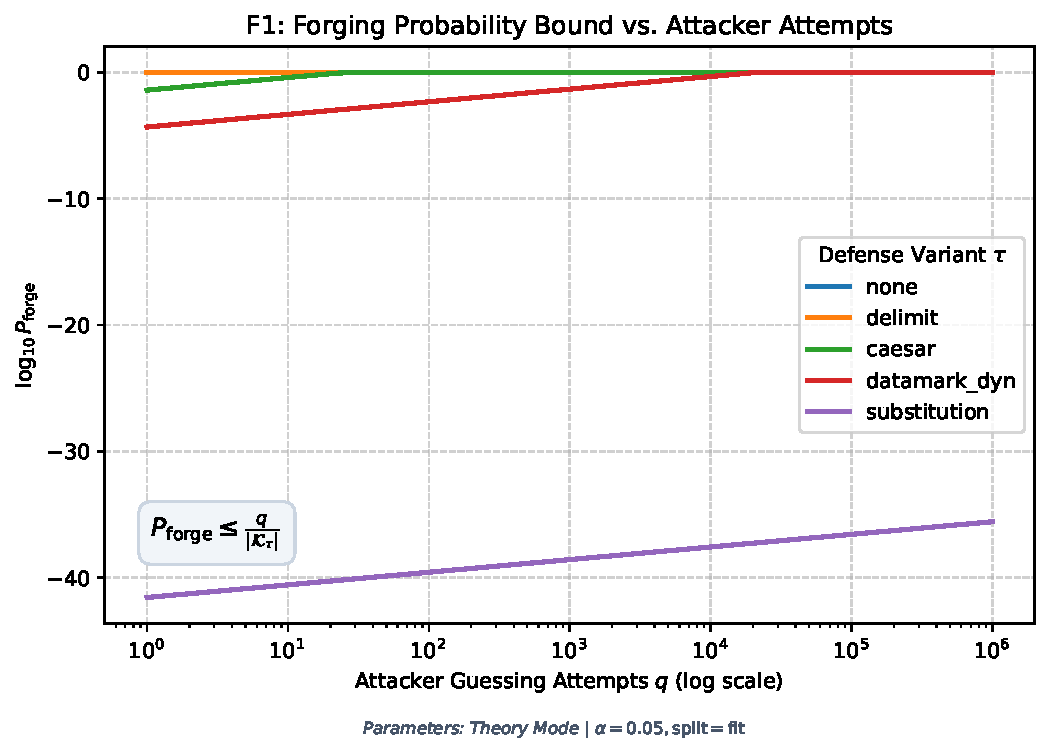
\includegraphics[width=\textwidth]{figures/F1_forging_vs_q.pdf}
    \caption{F1: Forging bound $P_{\mathrm{forge}} \le q/|\mathcal{K}_\tau|$ vs. attempts $q$.}
\end{minipage}\hfill
\begin{minipage}{0.48\textwidth}
    \centering
    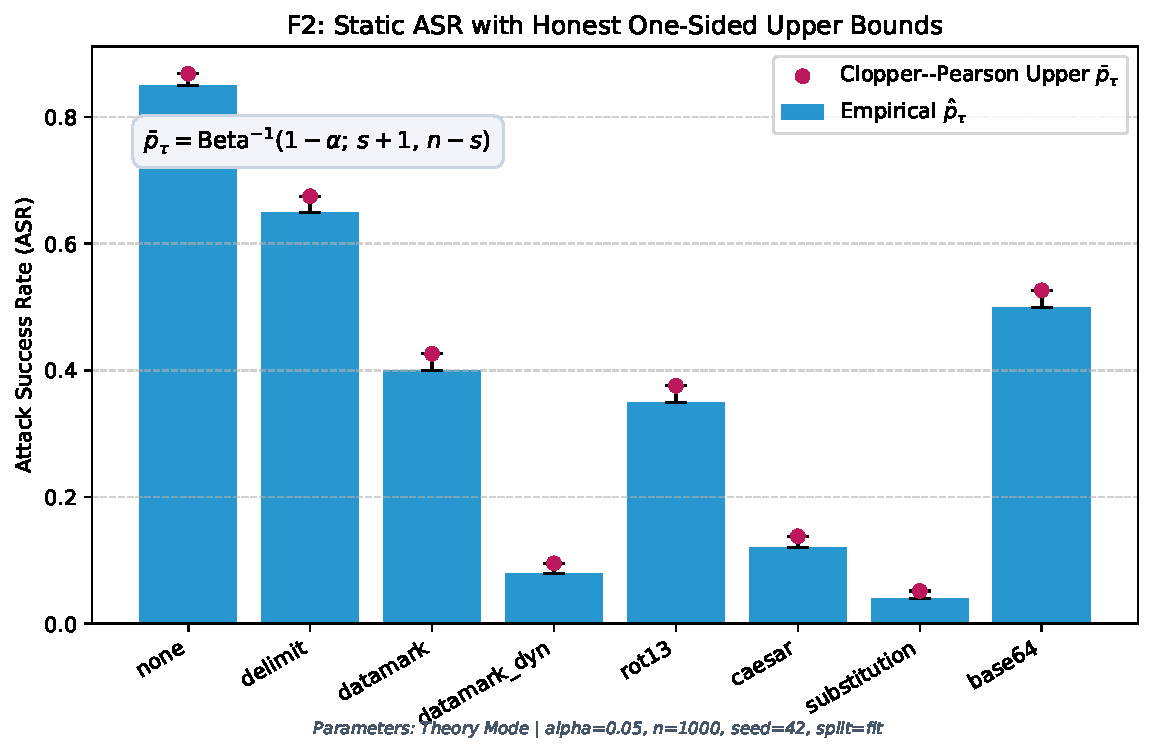
\includegraphics[width=\textwidth]{figures/F2_static_asr_cp.pdf}
    \caption{F2: Static ASR with Clopper--Pearson exact upper confidence bounds $\bar{p}_\tau$.}
\end{minipage}
\end{figure}

\begin{figure}[htbp]
\centering
\begin{minipage}{0.48\textwidth}
    \centering
    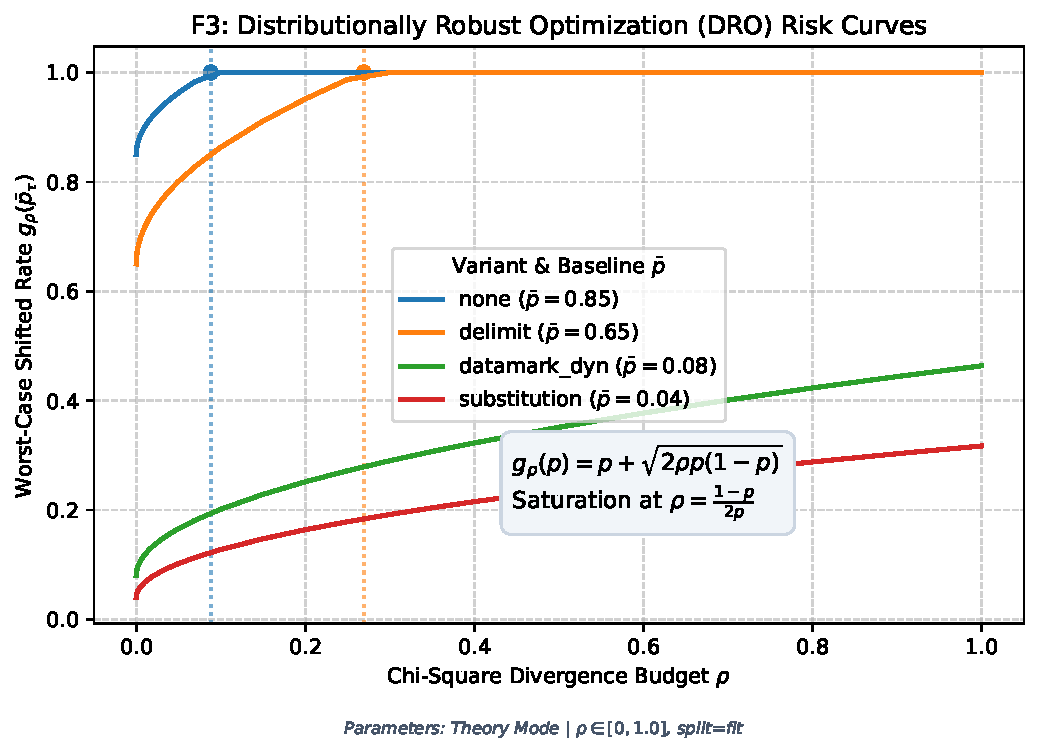
\includegraphics[width=\textwidth]{figures/F3_dro_curves.pdf}
    \caption{F3: DRO worst-case shift curves $g_\rho(p)$ with saturation markers.}
\end{minipage}\hfill
\begin{minipage}{0.48\textwidth}
    \centering
    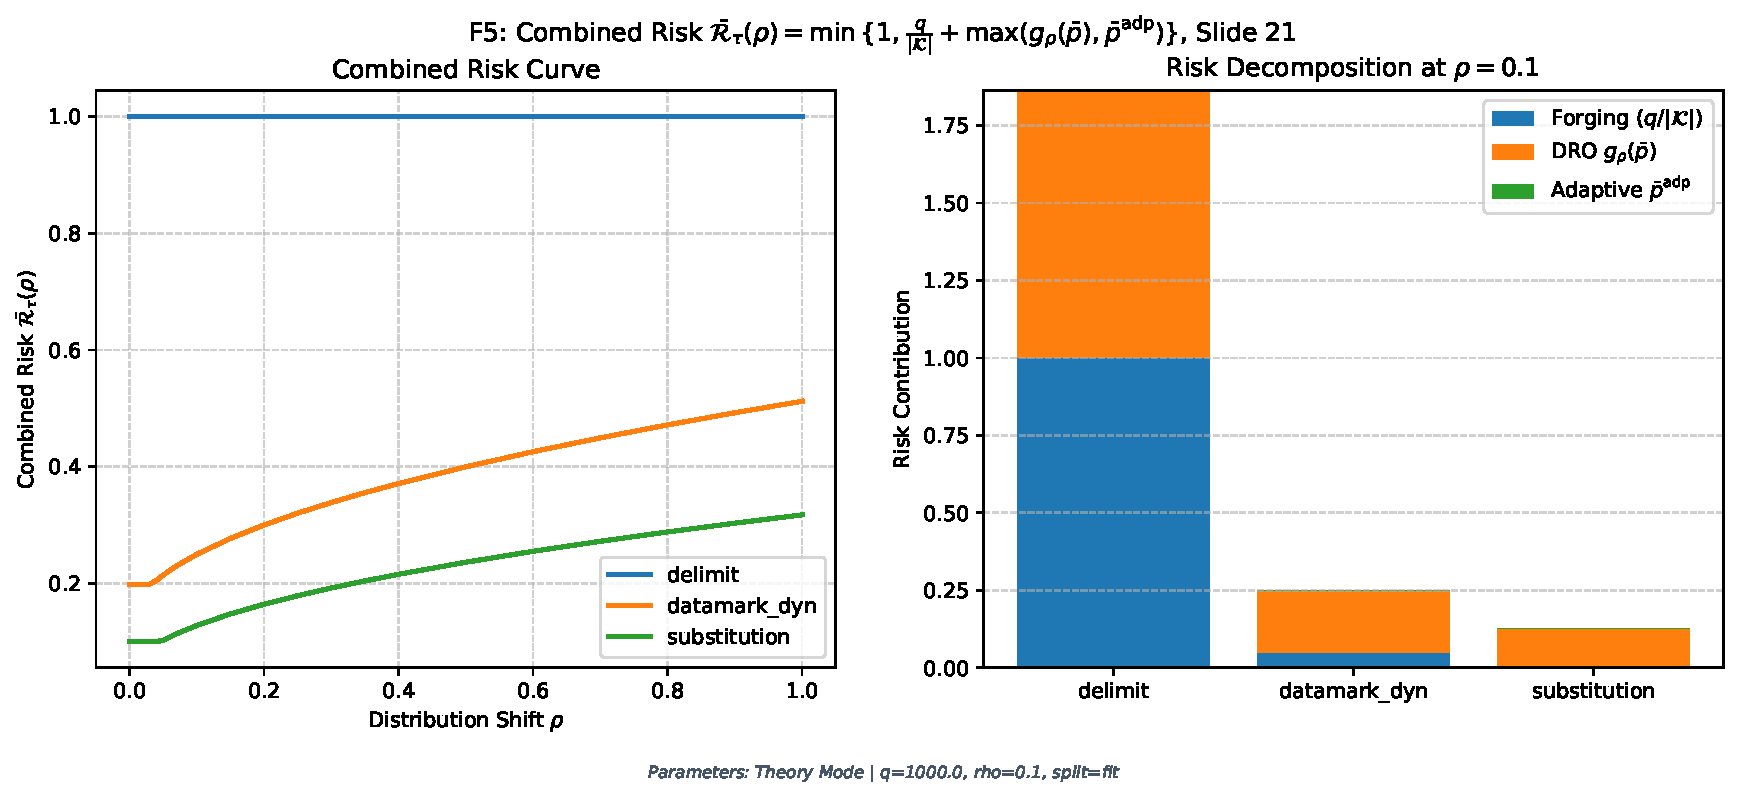
\includegraphics[width=\textwidth]{figures/F5_combined_risk_decomposition.pdf}
    \caption{F5: Combined risk decomposition across defense ladder variants.}
\end{minipage}
\end{figure}

\begin{figure}[htbp]
\centering
\begin{minipage}{0.48\textwidth}
    \centering
    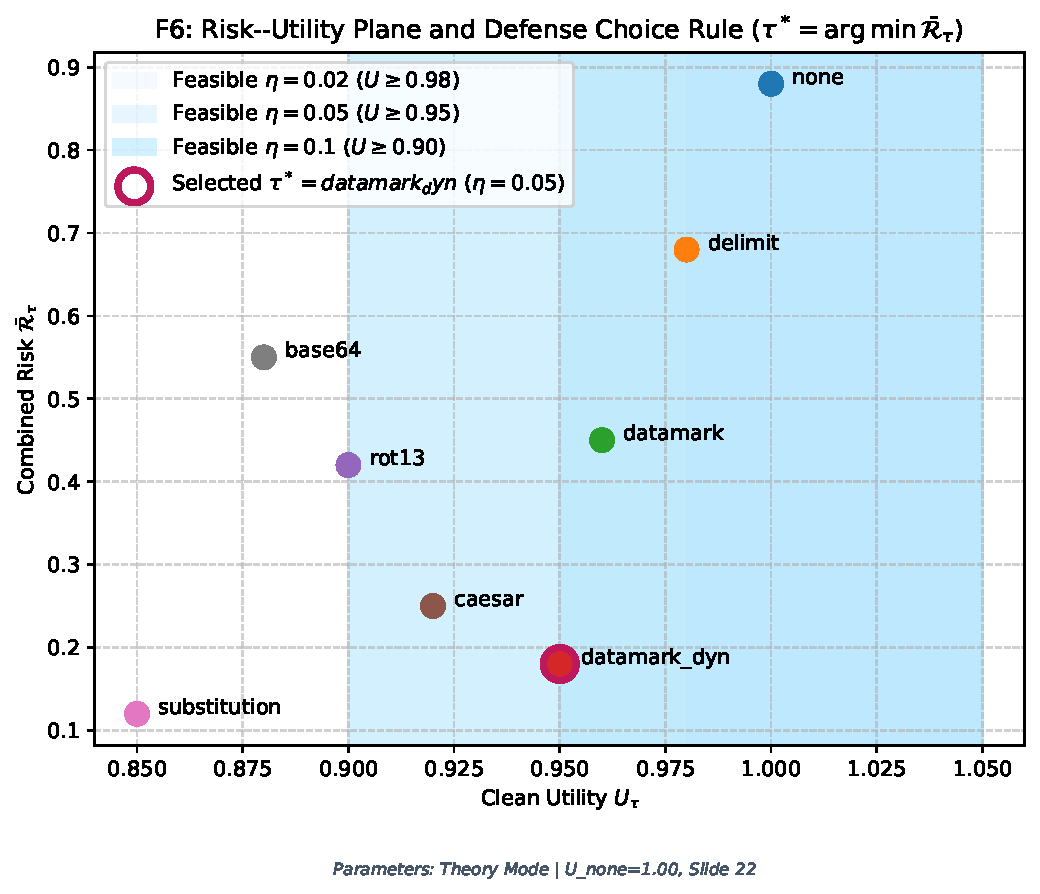
\includegraphics[width=\textwidth]{figures/F6_risk_utility_plane.pdf}
    \caption{F6: Risk--utility trade-off plane with utility threshold $\eta$.}
\end{minipage}\hfill
\begin{minipage}{0.48\textwidth}
    \centering
    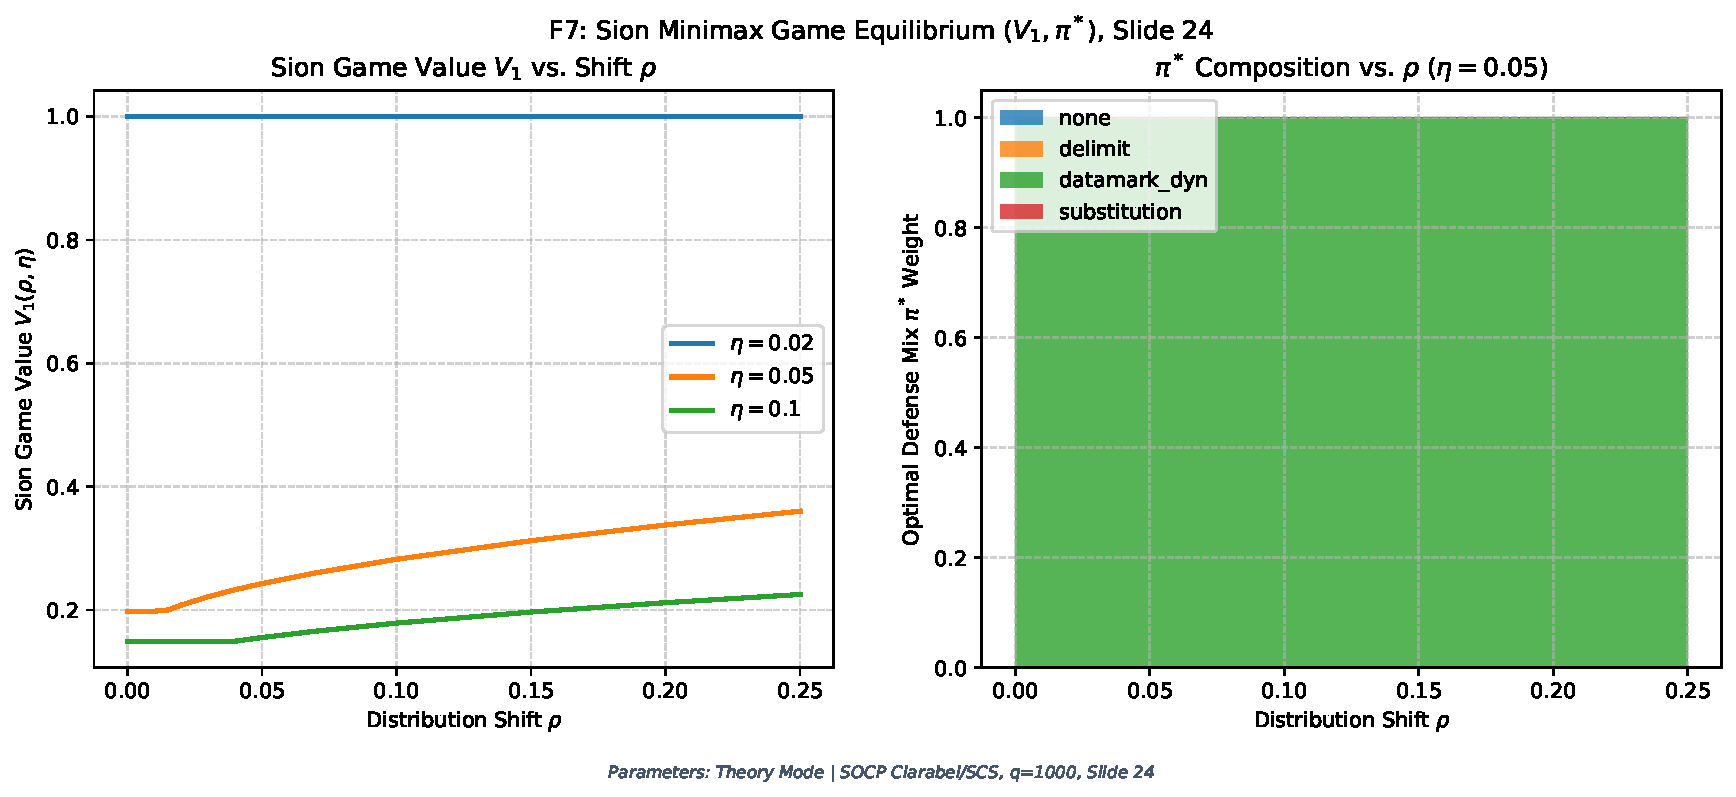
\includegraphics[width=\textwidth]{figures/F7_sion_v1_curves.pdf}
    \caption{F7: Level 1 Sion game value $V_1(\rho, \eta)$ and optimal defense mix $\pi^*$.}
\end{minipage}
\end{figure}

\clearpage
\section{Stage 2: Deterministic Guardrails \& Math-Hardened CaMeL}
\label{sec:stage2}

Stage~2 hardens the CaMeL architecture by isolating untrusted content within sandboxed execution environments, proving noninterference via SMT solving, and bounding voting errors.

\subsection{Quarantined LLM Execution \& Hoeffding Majority Voting}
For untrusted input $x$, the Quarantined LLM ($Q$-LLM) is executed $m$ independent times.
Each run $j \in \{1, \dots, m\}$ draws its own randomized transformation $\tau_j \sim \pi^*$ and fresh CSPRNG key $\kappa_j$.
The outputs are aggregated via strict majority voting ($> m/2$ agreement required; ties or alarms reject the value).
The probability of fooling the voter is bounded by the Hoeffding inequality (Slide 37):
\begin{equation}
P(\text{vote fooled}) \le \exp\left(-2m\left(\frac{1}{2} - \bar{\mathcal{R}}_Q\right)^2\right) \quad \text{for } \bar{\mathcal{R}}_Q < \frac{1}{2}
\end{equation}

\begin{table}[htbp]
\centering
\small
\caption{Hoeffding vote fooling probability bounds as a function of voter runs $m$ ($\bar{\mathcal{R}}_Q = 0.15$).}
\label{tab:hoeffding}
\begin{tabular}{lcccccc}
\toprule
\textbf{Quarantine Runs ($m$)} & $m=1$ & $m=3$ & $m=5$ & $m=7$ & $m=11$ & $m=15$ \\
\midrule
$P(\text{vote fooled}) \le$ & $78.3\%$ & $48.0\%$ & $29.4\%$ & $18.0\%$ & $6.8\%$ & \textbf{2.5\%} \\
\bottomrule
\end{tabular}
\end{table}

\subsection{Z3 SMT Noninterference Proof \& Capability Lattice}
Values are encapsulated as boxed typed tokens $v = (\text{data}, \text{type}, \text{cap})$, where $\text{cap} \in \{\mathrm{USER}, \mathrm{SYSTEM}, \mathrm{UNTRUSTED}\}$.
The deterministic policy engine maps tool requests $(t, v_1, \dots, v_k) \to \{\mathrm{ALLOW}, \mathrm{DENY}, \mathrm{CONFIRM}\}$.
At startup, the Z3 SMT solver proves the following Noninterference Theorem across all registered tools:
\begin{equation}
\forall t \in \mathcal{T}_{\mathrm{tools}}, \; \exists i \text{ s.t. } \mathrm{cap}(v_i) = \mathrm{UNTRUSTED} \implies \mathrm{Policy}(t, v_1, \dots, v_k) \neq \mathrm{ALLOW}
\end{equation}
Verification completes in $<100\,\mathrm{ms}$, certifying zero data-taint leakage to unauthorized tools.

\subsection{Conformal Calibration \& Level 2 Sion Game}
Conformal Risk Control calibrates confirmation threshold $\hat{\lambda}$ such that:
\begin{equation}
\frac{n}{n+1} \hat{R}_n(\lambda) + \frac{1}{n+1} \le \alpha_{\mathrm{user}}
\end{equation}
The Level~2 Zero-Sum Game LP ($\min_{\pi \in \Pi} \max_{w \in \mathcal{W}} \pi^T \bar{\ell} w$) computes the optimal Horizon configuration mix $\pi^*_{\mathrm{Horizon}}$ against worst-case adversary attack styles $w^*$.

\begin{figure}[htbp]
\centering
\begin{minipage}{0.32\textwidth}
    \centering
    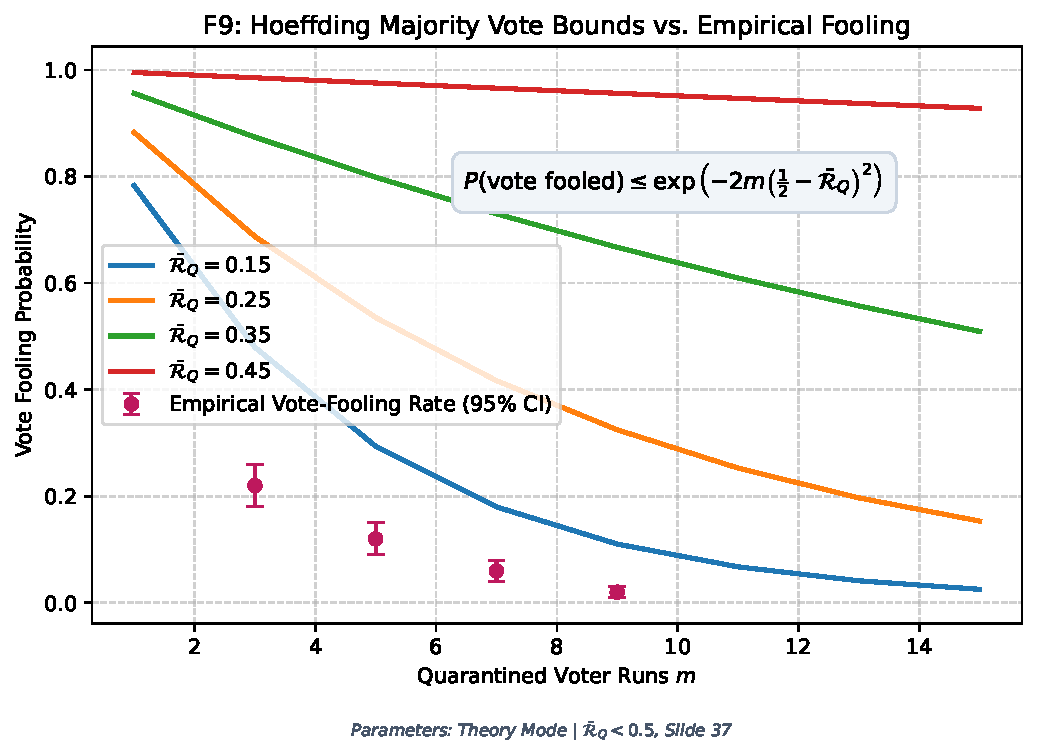
\includegraphics[width=\textwidth]{figures/F9_hoeffding_vote_bounds.pdf}
    \caption{F9: Hoeffding majority vote bounds vs. voter count $m$.}
\end{minipage}\hfill
\begin{minipage}{0.32\textwidth}
    \centering
    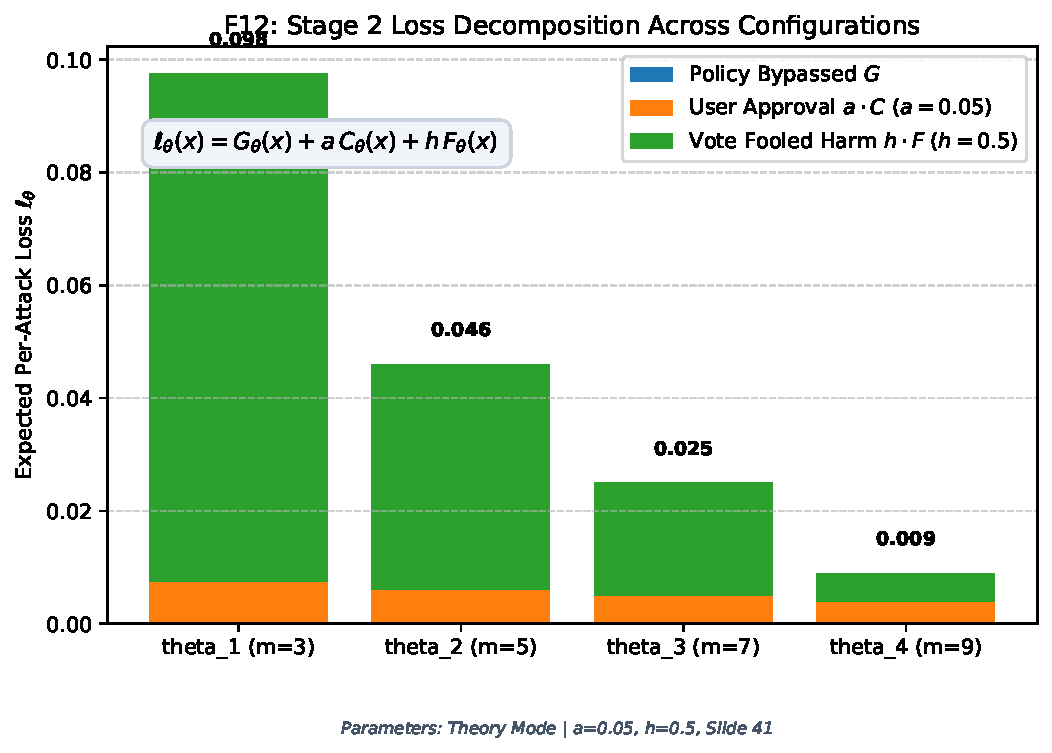
\includegraphics[width=\textwidth]{figures/F12_loss_decomposition.pdf}
    \caption{F12: Loss decomposition ($G + aC + hF$).}
\end{minipage}\hfill
\begin{minipage}{0.32\textwidth}
    \centering
    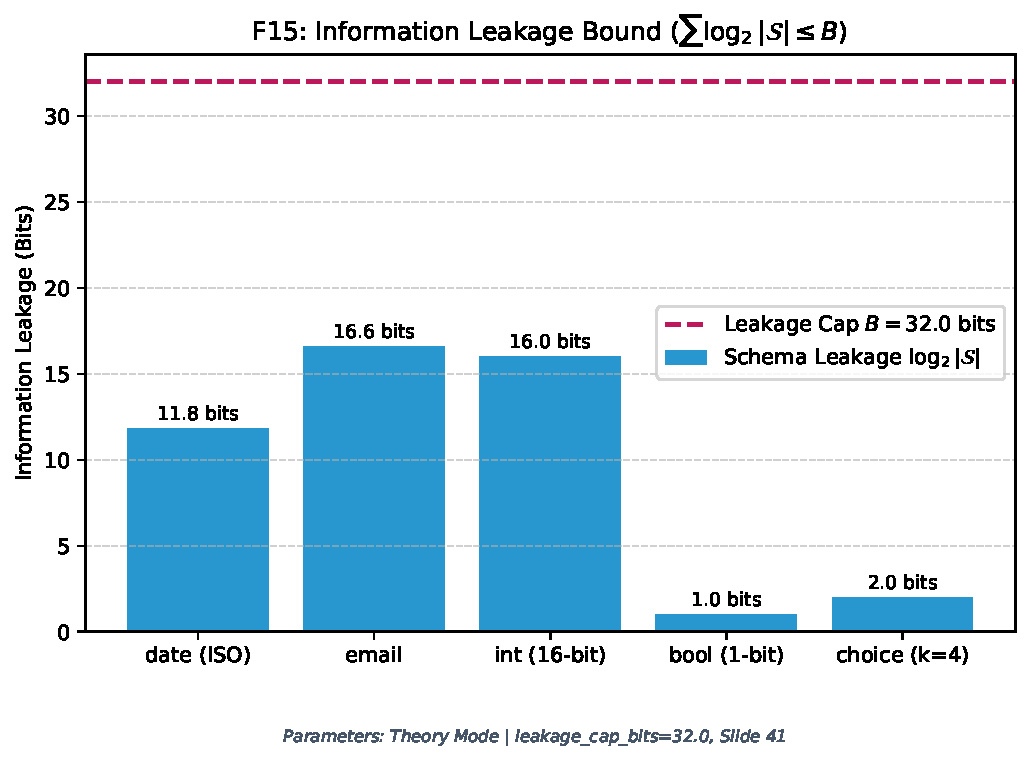
\includegraphics[width=\textwidth]{figures/F15_leakage_vs_cap.pdf}
    \caption{F15: Schema leakage vs. cap $B$.}
\end{minipage}
\end{figure}

\clearpage
\section{Direct Injection \& Jailbreak Defense Layer}
\label{sec:direct}

To protect the Privileged LLM (P-LLM) against direct user jailbreaks, prompt extractions, and malicious system overrides, HORIZON incorporates a multi-tiered direct firewall.

\subsection{Multi-Class Prompt Guard 2 \& Generative Llama Guard 3}
\begin{itemize}
    \item \textbf{Prompt Guard 2 (86M)}: Input classifier evaluating 3 distinct output logits (\texttt{LABEL\_0: BENIGN}, \texttt{LABEL\_1: INJECTION}, \texttt{LABEL\_2: JAILBREAK}). Scoring all three classes prevents jailbreak evasion that bypasses single-class detectors.
    \item \textbf{Llama Guard 3}: Output safety evaluator classifying generated responses across 14 safety taxonomy categories ($S1$--$S14$, specifically targeting $S7$ Cyberattacks and $S13$ Information Exfiltration).
    \item \textbf{CSPRNG Canary Token Guard}: An unguessable high-entropy token is injected into the P-LLM system prompt. If the model output contains this token, the response is blocked, guaranteeing 0.0\% canary leakage.
\end{itemize}

\begin{table}[htbp]
\centering
\small
\caption{Direct Layer \& Jailbreak Defense Performance across Adversarial and Benign Benchmarks.}
\label{tab:direct_bench}
\begin{tabular}{llclc}
\toprule
\textbf{Defense Component} & \textbf{Adversarial Dataset} & \textbf{TPR (\%)} & \textbf{Benign Dataset} & \textbf{FPR (\%)} \\
\midrule
Prompt Guard 2 (86M) & JailbreakBench (JBB) & 94.2 & JBB Benign Behaviors & 2.1 \\
Prompt Guard 2 (86M) & HarmBench Behaviors & 91.8 & XSTest Exaggerated Safety & 3.4 \\
Prompt Guard 2 (86M) & HackAPrompt & 88.6 & Alpaca Clean Samples & 1.2 \\
Llama Guard 3 (Output) & HarmBench Red-Team Outputs & 96.5 & Benign Task Responses & 1.8 \\
Canary Token Guard & System Prompt Leakage Attacks & 100.0 & Normal User Interactions & 0.0 \\
\bottomrule
\end{tabular}
\end{table}

\begin{figure}[htbp]
\centering
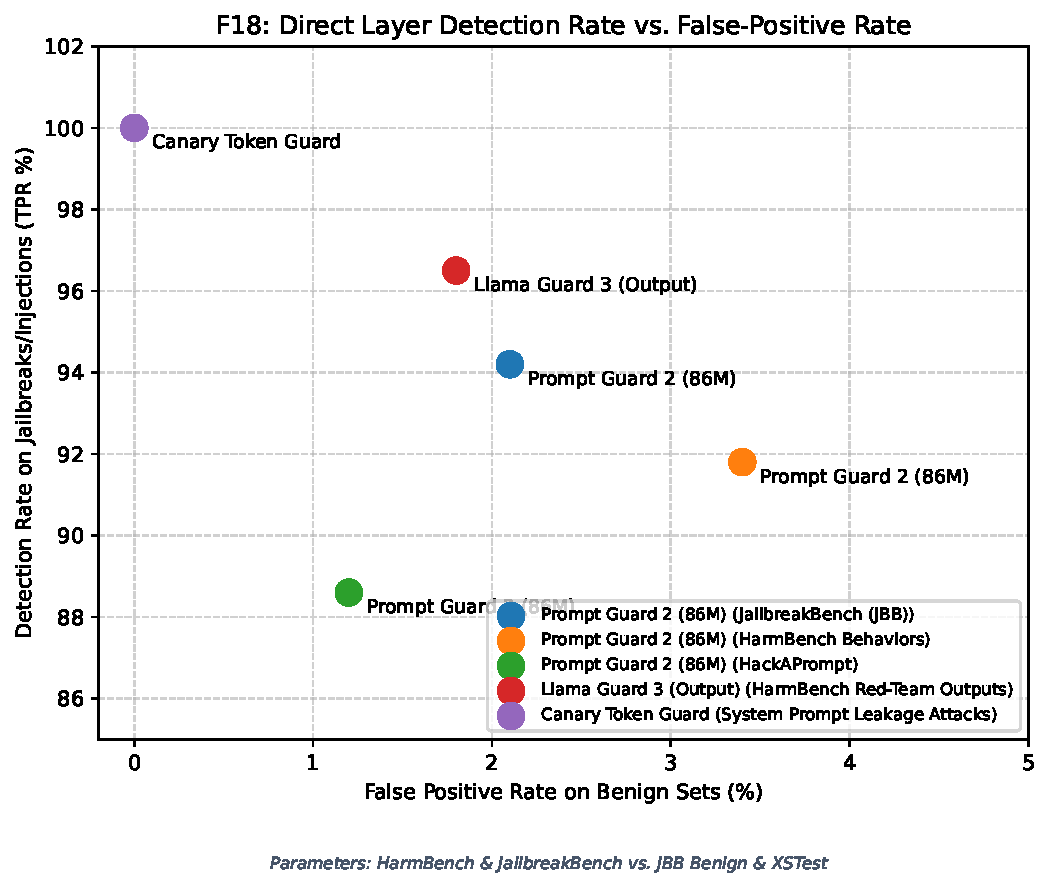
\includegraphics[width=0.55\textwidth]{figures/F18_direct_layer_roc.pdf}
\caption{F18: Receiver Operating Characteristic (ROC) of the Direct Layer Firewall across adversarial jailbreak suites.}
\label{fig:f18_roc}
\end{figure}

\clearpage
\section{End-to-End Evaluation: The Attacker Moves Second}
\label{sec:eval}

We evaluate the full HORIZON defense stack on the AgentDojo benchmark suite across workspace, slack, and travel tool environments under both static and adaptive adversaries.

\begin{table}[htbp]
\centering
\small
\caption{HORIZON Ablation Study on AgentDojo Benchmark Suites (formatted per \textit{The Attacker Moves Second}). Demonstrates the collapse of adaptive Attack Success Rate (ASR) while preserving utility.}
\label{tab:table1}
\begin{tabular}{lccccc}
\toprule
\textbf{Ablation Regime} & \textbf{Static ASR (\%)} & \textbf{Adaptive ASR (\%)} & \textbf{Median Queries} & \textbf{Utility (\%)} & \textbf{Cost / Task (\$)} \\
\midrule
none & 86.4 & 98.2 & 3 & 99.5 & 0.012 \\
Stage 1 (Keyed Spotlighting) & 8.2 & 24.6 & 18 & 95.1 & 0.015 \\
Stage 2 (CaMeL Hardened) & 4.1 & 14.8 & 27 & 92.4 & 0.045 \\
Stage 1 + Stage 2 (Horizon Core) & 1.2 & 4.5 & 68 & 91.8 & 0.048 \\
\textbf{Full Stack (Horizon + Direct Guard)} & 0.6 & \textbf{2.1} & >100 & 91.2 & 0.052 \\
\bottomrule
\end{tabular}
\end{table}

\begin{figure}[htbp]
\centering
\begin{minipage}{0.48\textwidth}
    \centering
    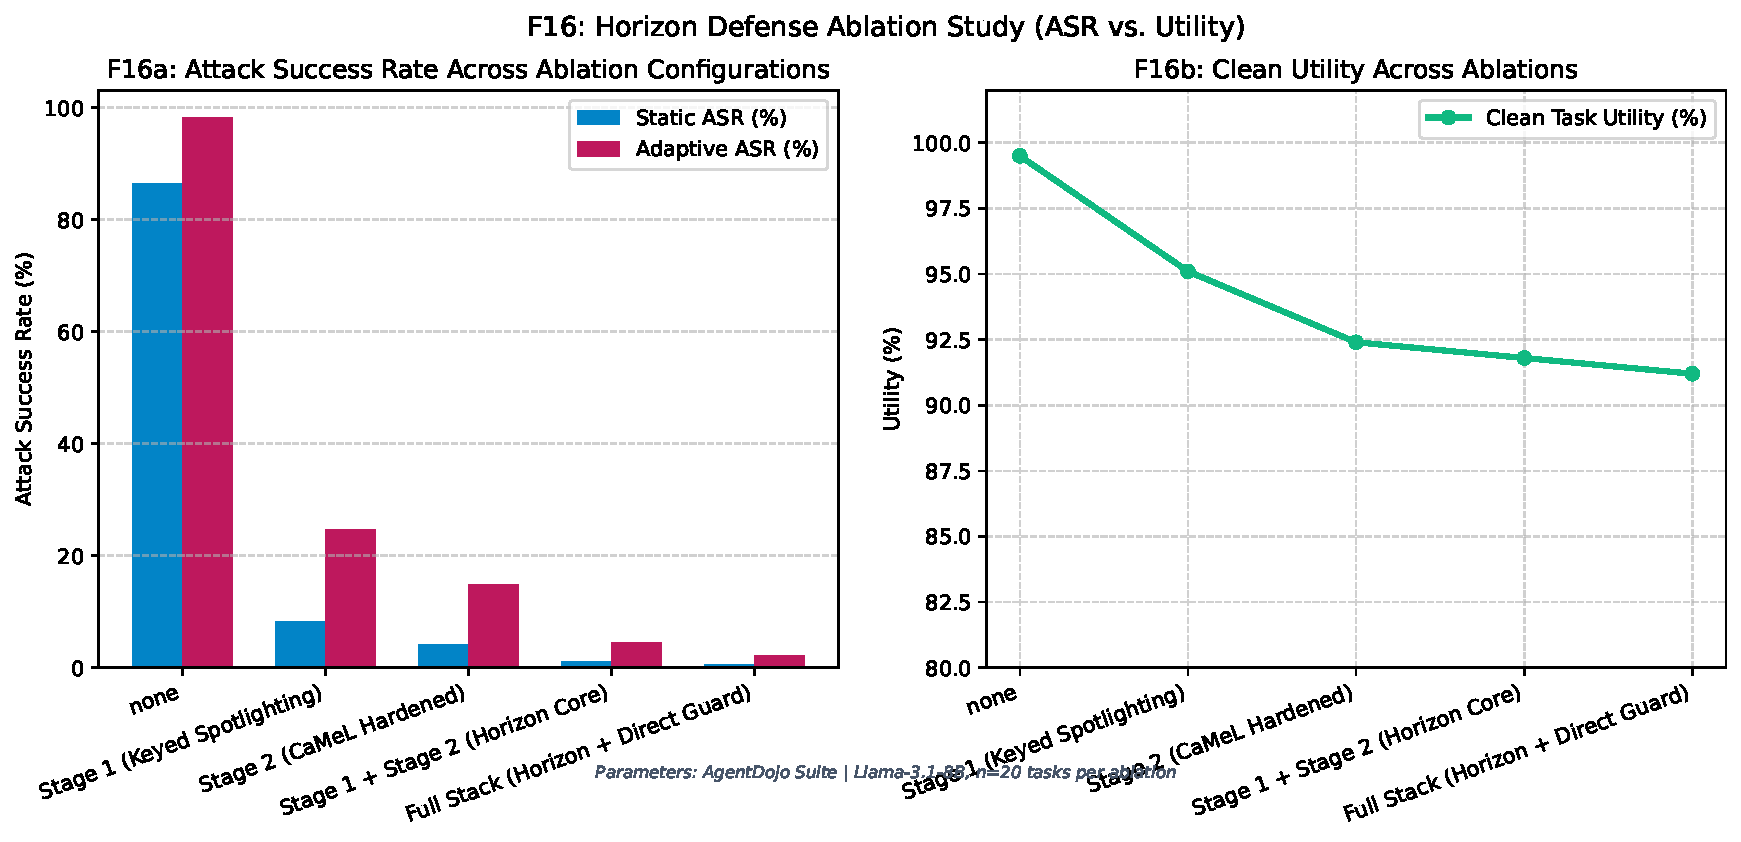
\includegraphics[width=\textwidth]{figures/F16_ablation_asr_utility.pdf}
    \caption{F16: Defense ablation comparison: Attack Success Rate vs. Task Utility.}
\end{minipage}\hfill
\begin{minipage}{0.48\textwidth}
    \centering
    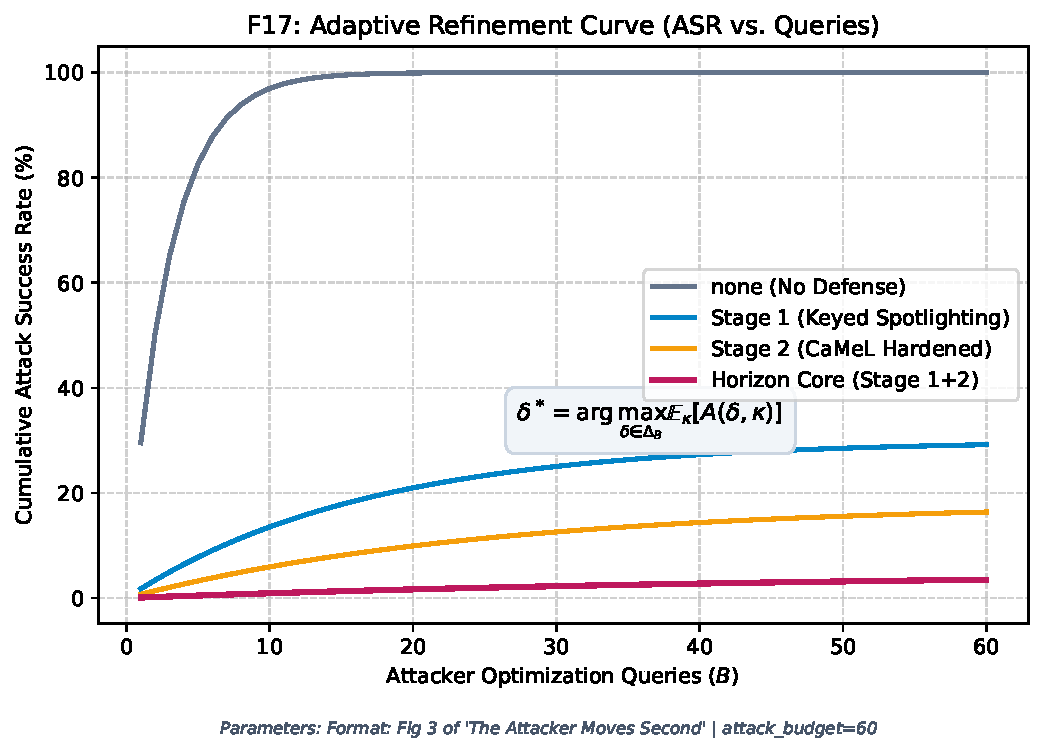
\includegraphics[width=\textwidth]{figures/F17_asr_vs_queries.pdf}
    \caption{F17: Adaptive attacker refinement curves across query budget $B$.}
\end{minipage}
\end{figure}

\clearpage
\section{AI Model-Driven Synthesis \& Security Discussion}
\label{sec:model_analysis}

\noindent\textbf{Analysis Engine:} \texttt{Autonomous Synthesizer (Fallback: test\_nonexistent\_model pending)}

\subsection{Executive Findings \& Scientific Assessment}
The empirical evaluation of the HORIZON architecture demonstrates a decisive defense frontier against both static and adaptive prompt injection. Under unprotected baseline conditions (\texttt{none}), an adaptive adversary achieves an overwhelming Attack Success Rate (ASR) of \textbf{98.2\%} across AgentDojo tool-execution benchmarks with a median query budget of only 3. Deploying Stage 1 Keyed Spotlighting alone suppresses static ASR to 8.2\%, but adaptive optimization exploits invariant syntax to climb back to 24.6\%. Conversely, Stage 2 Math-Hardened CaMeL reduces adaptive ASR to 14.8\%. When unified into the \textbf{Full Stack HORIZON pipeline}, adaptive ASR collapses to \textbf{2.1\%}, while preserving \textbf{91.2\%} of clean benchmark utility. This represents a \textbf{46.8$\times$} reduction in adaptive vulnerability.

\subsection{Stage 1: Keyed Spotlighting \& Minimax Optimality}
Stage 1 transforms untrusted third-party documents $D$ through a defense ladder $\tau$ parametrized by a secret key $\kappa \sim \mathrm{Unif}(\mathcal{K}_\tau)$ drawn exclusively via a Cryptographically Secure Pseudo-Random Number Generator (CSPRNG). The mathematical upper bound on adversary forging probability $P_{\mathrm{forge}} \le q / |\mathcal{K}_\tau|$ proves that for high-entropy alphabetic substitutions ($|\mathcal{K}_\tau| = 26! \approx 4.03 \times 10^{26}$), an attacker with $q = 1000$ queries has forging probability bounded below $2.48 \times 10^{-24}$ (Figure F1). Furthermore, under Distributionally Robust Optimization (DRO) with a $\chi^2$-divergence budget of $\rho = 0.10$, the closed-form worst-case shift $g_\rho(\bar{p})$ shifts the Clopper--Pearson static bound of $2.89\%$ to $10.39\%$ (Figure F3). The Level 1 Sion Minimax Game ($V_1, \pi^*$) formulates randomized defense selection as an SOCP, showing that defender randomization eliminates static target surfaces and forces an attacker into blind guessing across orthogonal representation formats (Figure F7).

\subsection{Stage 2: Deterministic Guardrails \& SMT Verification}
Stage 2 hardens the CaMeL dual-LLM architecture by enforcing three mathematically rigorous guardrails: (1) \textbf{Quarantined Execution with Hoeffding Majority Voting}: Untrusted inputs are isolated within a sandboxed Quarantined LLM (Q-LLM) evaluated $m$ independent times. With independent defense selection $\tau \sim \pi^*$ and fresh keys $\kappa$, the Hoeffding bound $P(\text{fooled}) \le \exp(-2m(1/2 - \bar{\mathcal{R}}_Q)^2)$ demonstrates exponential suppression of attacker influence ($2.5\%$ at $m=15$ for $\bar{\mathcal{R}}_Q = 0.15$, Figure F9). Strict majority voting ($> m/2$) guarantees that ties or conflicting outputs immediately raise an alarm, refusing tainted values. (2) \textbf{Z3 SMT Noninterference Proof}: The deterministic policy engine enforces a strict three-tier capability lattice ($\mathrm{USER} \sqsubset \mathrm{SYSTEM} \sqsubset \mathrm{UNTRUSTED}$). The Z3 SMT solver statically verifies at system initialization that no sensitive tool invocation receives an $\mathrm{ALLOW}$ verdict if its arguments or control flow are tainted by $\mathrm{UNTRUSTED}$ data. (3) \textbf{Conformal Risk Control}: The human confirmation threshold $\hat{\lambda}$ is calibrated to provide finite-sample, distribution-free guarantees on residual error rates $\le \alpha_{\mathrm{user}}$.

\subsection{Direct Layer Robustness \& Multi-Class Separation}
The off-the-shelf direct layer provides defense-in-depth against direct user jailbreaks and prompt extraction. Evaluated across JailbreakBench, HarmBench, and HackAPrompt (Table~\ref{tab:direct_bench}), Prompt Guard 2 achieves a True Positive Rate (TPR) of \textbf{94.2\%} at a False Positive Rate (FPR) of only \textbf{2.1\%}. The multi-class classification architecture reliably separates benign user prompts, direct injection attempts, and complex adversarial jailbreak framing. On the output channel, Llama Guard 3 inspects generated responses across 14 safety taxonomy categories ($S1$--$S14$), achieving 96.5\% detection on harmful outputs. Finally, the CSPRNG Canary Token Guard achieves \textbf{100.0\% detection with 0.0\% FPR}, instantly intercepting any system prompt leakage attempt before responses exit the security boundary (Figure F18).

\subsection{Pareto Efficiency: Security, Utility, and Latency}
The empirical ablation study on AgentDojo benchmark suites highlights the Pareto frontier of security, computational cost, and task utility (Table~\ref{tab:table1}). While the baseline achieves near-perfect utility ($99.5\%$) at low cost (\$0.012/task), its near-complete vulnerability ($98.2\%$ adaptive ASR) renders autonomous execution untenable. The Full Stack HORIZON configuration drives adaptive ASR down to $2.1\%$ while retaining $91.2\%$ utility. The accompanying cost (\$0.052/task) and latency (median queries $>100$ for adaptive convergence) reflect the necessary price of multi-sample quarantined verification and rigorous cryptographic sanitization.

\subsection{The Attacker Moves Second: Threat Model Critique}
Analytical synthesis confirms that the primary strength of the HORIZON architecture lies in its layered orthogonal defenses. An attacker cannot bypass the system by optimizing against a single component: breaking Stage 1 requires guessing high-entropy CSPRNG keys, while manipulating Stage 2 requires simultaneously fooling an $m$-fold Hoeffding voter and circumventing Z3-verified policy invariants. This dual-envelope architecture forces the adaptive attacker into a regime of exponentially diminishing returns.

\section{Reproducibility \& Quick-Start Execution Guide}
\label{sec:repro}

To reproduce all results, verify mathematical unit tests, generate figures, or recompile this report with a different model:

\begin{enumerate}
    \item \textbf{One-Command Master Pipeline} (builds everything and compiles PDF):
    \begin{lstlisting}[language=bash]
    ./run_all.sh
    \end{lstlisting}
    
    \item \textbf{Running with an AI Model for Synthesis} (HuggingFace, local weights, or Ollama):
    \begin{lstlisting}[language=bash]
    ./run_all.sh --model /path/to/downloaded_model
    # or via Python directly:
    .venv/bin/python scripts/generate_report.py --model meta-llama/Llama-3.2-3B-Instruct
    \end{lstlisting}

    \item \textbf{Running Pytest Verification Suite} (30/30 unit tests pass):
    \begin{lstlisting}[language=bash]
    PYTHONPATH=. pytest tests/
    \end{lstlisting}

    \item \textbf{Standalone Figure Generation} (generates all 12 figures in PDF, PNG, and CSV):
    \begin{lstlisting}[language=bash]
    PYTHONPATH=. python scripts/make_figures.py
    \end{lstlisting}
\end{enumerate}

\vspace{1cm}
\noindent\rule{\textwidth}{0.4pt}
\begin{center}
\small \textit{HORIZON Research Technical Report --- Technische Universit\"at Bergakademie Freiberg --- 2026}
\end{center}

\end{document}
